% This file is isea.tex.  It contains the formatting instructions for and acts as a template for submissions to ISEA 2015.  It is based on the ICCC  formats and instructions.  It uses the files isea.sty, isea.bst and isea.bib, the first two of which also borrow from AAAI IJCAI formats and instructions.
% Modified from ICCC.tex by B. Bogart

\documentclass[letterpaper]{article}
\usepackage{isea}
\usepackage[pdftex]{graphicx}
\usepackage{times}
\usepackage{helvet}
\usepackage{courier}
\usepackage[numbers]{natbib}
\pdfinfo{
/Title (Scaling with multiple network namespaces in a single application)
/Author (PJ Waskiewicz)}
% The file isea.sty is the style file for ISEA 2015 proceedings.
%
\title{Scaling With Multiple Network Namespaces in a Single Application}
\author{PJ Waskiewicz\\
Principal Engineer at NetApp\\
Portland, OR, USA\\
pj.waskiewicz@netapp.com\\
\newline
\newline
}
\setcounter{secnumdepth}{0}

\begin{document} 
\maketitle
\begin{abstract}
Namespaces and containers seem to be the rage today, but it’s not typical for large applications to use them directly. Rather, applications rely on frameworks such as LXC and/or Docker to manage the containers they run in.

This paper will focus on how a large application can utilize the network namespace framework, and how it can use large numbers of namespaces to partition up the underlying network infrastructure within the application. An overview of parts of the application architecture using the namespaces will be covered, showing the use cases driving the need for namespaces. Lessons learned around scalability and performance bottlenecks in the kernel will be shared.

Ultimately this paper will propose further improvements to the namespace framework for better programmatic management of namespaces within the kernel from userspace, as well as attention to increased scalability and efficiency of networking within the namespaces.
\end{abstract}

\section{Keywords}

networking, kernel, containers, namespaces, scaling, cloud

\section{Introduction}
The ongoing evolution of the datacenter towards cloud-based infrastructure continues to present interesting challenges to existing applications. These existing solutions, e.g. storage appliances, work to serve multiple tenants within a computing domain. However, when the infrastructure around these solutions evolves into a cloud-based, partitioned environment, these solutions must also evolve.

When an application has core logic that needs to span multiple, separate network environments, it must become container/network-namespace aware. The Linux kernel exposes an API to create and manage network namespaces within an application. This paper will focus on this API for the following:
\begin{itemize}
\item How to create and manage the lifecycle of a network namespace within a complex application
\item How to track and process multiple network connections across multiple network namespaces in an efficient and scalable manner
\item What limitations exist in this API that makes lifecycle management a challenge, along with proposals on how to improve the API for better lifecycle management
\item Scalability issues encountered, how these were addressed, and proposals around scalability testing to prevent regressions
\end{itemize}

\section{The Need For Multiple Network Namespaces}
Typical network-based storage applications have various layers of the core logic separated from one another. For example, the volume database containing metadata mappings to underlying block or object data is completely separated from the networking core, since they share no common functionality. In Figure \ref{app-overview}, one can see an example of how different components are separated from one another. Core logic for volume tracking in one functional area, thread management in another area, the iSCSI or Fibre Channel protocol stack handled elsewhere, and ultimately the underlying networking being handled by the underlying OS.

Consider a public or private cloud environment, where "legacy" datacenter models migrate pieces of their infrastructure into that cloud environment. A typical storage application as Figure \ref{app-overview} could have all storage volumes from that legacy datacenter migrated as one tenant. However, multiple tenants may have conflicting environment configurations, such as IP address range collisions, different routing hierarchies, or different VLAN segregation within their respective network domains. By creating a completely new network stack inside of a network namespace for each of these legacy environments, the containers can fully segregate the network environments from one another, and avoid any changes to the legacy datacenter configuration.

When an application architecture such as this needs to fit into an environment where the networking is the component that needs to support multiple containers, one can observe that using Docker or LXC is not sufficient. They are not sufficient since those deal with containerizing an entire application, not pieces of an application. Let us consider some different approaches to try and solve this problem of supporting multiple network stacks within an application.

\begin{figure}[h]
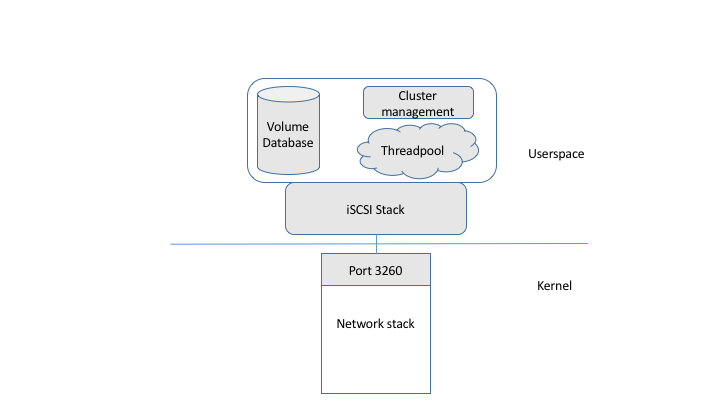
\includegraphics[width=3.31in]{standard-app-overview.png}
\caption{High-level architecture of application.}
\label{app-overview}
\end{figure}

\subsection{Approach 1: Fork}

\subsection{Approach 2: Thread per-network namespace}

\subsection{Approach 3: Global file descriptor per-network namespace}

\section{Network Namespace Management}

\subsection{Identifying Different Namespaces}

\subsection{Returning to the Base}

\subsection{Efficient Namespace Switching}

\section{Network Namespace Scalability}

\begin{figure}[h]
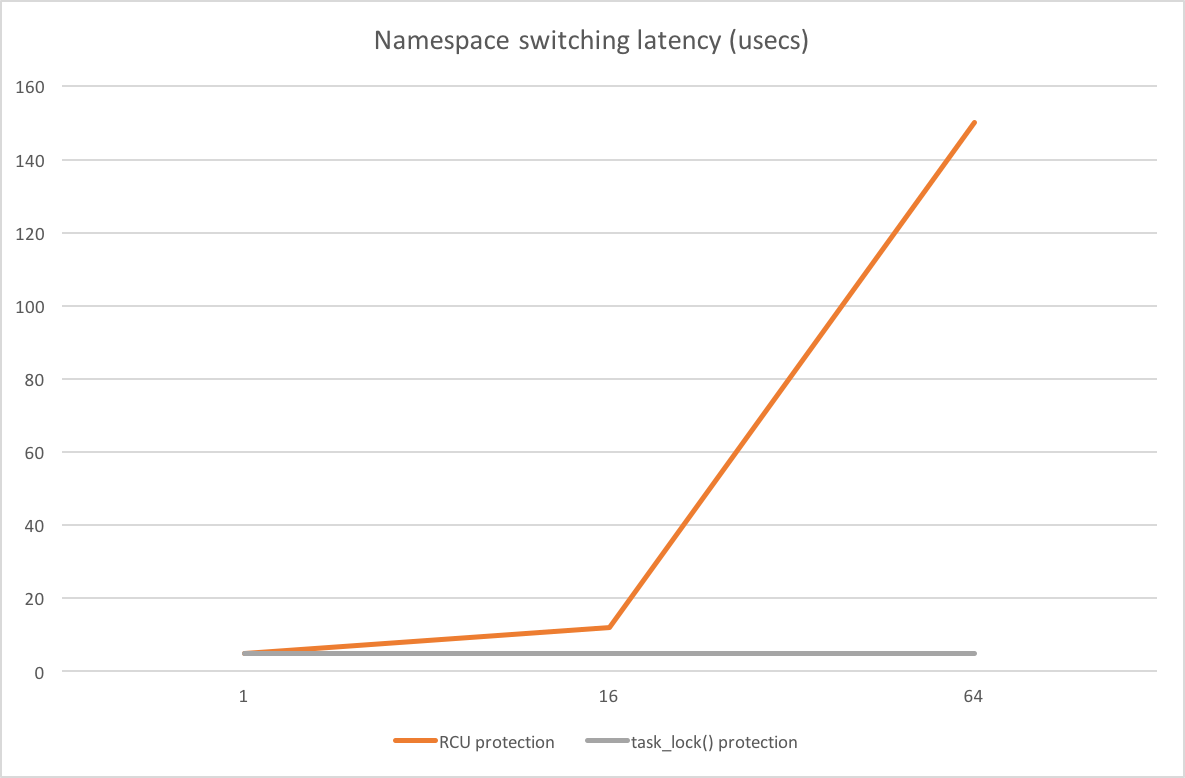
\includegraphics[width=3.31in]{close-up-latency.png}
\caption{Network namespace switching latency, close-up}
\label{close-latency}
\end{figure}

\section{Proposed Improvements}

\subsection{More Uniqueness}

\subsection{Performance Regression Testing}

\section{Conclusion}
The network namespace API in the Linux kernel provides a very powerful framework for applications to take advantage of. This allows large applications that need to span multiple network namespaces to not require complete architectural upheavals of core logic outside of the networking layers. Using some clever tricks and techniques, the namespace switching and lifecycle management can be very efficient. Moving forward, we believe there is still more that can be done to improve this API, and make it even more powerful as containers continue to grow in popularity and wide-spread deployment across the computing industry.

\section{Acknowledgments}
We would like to acknowledge the engineers who contributed to this network namespace application design: Joe Roback, Carl Seelye, Tom Distler, Jared Cantwell, and Marshall McMullen.

We would also like to acknowledge the Netdev1.2 selection committee for inviting us to submit and present this paper.

\bibliographystyle{pj-netdev-1.2}
\bibliography{pj-netdev-1.2}

\section{Author Biography}
PJ Waskiewicz is a Principal Software Engineer at NetApp in the SolidFire division. Prior to SolidFire/NetApp, PJ worked for many years as a network kernel engineer and device driver developer in the Networking Division of Intel. There he maintained and helped create the igb, ixgbe, and i40e wired Ethernet network drivers, as well as the initial Tx multiqueue support in the network stack, and Data Center Bridging support in the Linux kernel. He also worked in Intel's Open Source Technology Center on the x86 kernel tree, enabling advanced features in the Broadwell and Skylake microarchitectures.

\end{document}
